\vspace{-2.5ex}
\section{Related Work}

\begin{figure*}[!t]
\vspace{-0.5ex}
\centering
  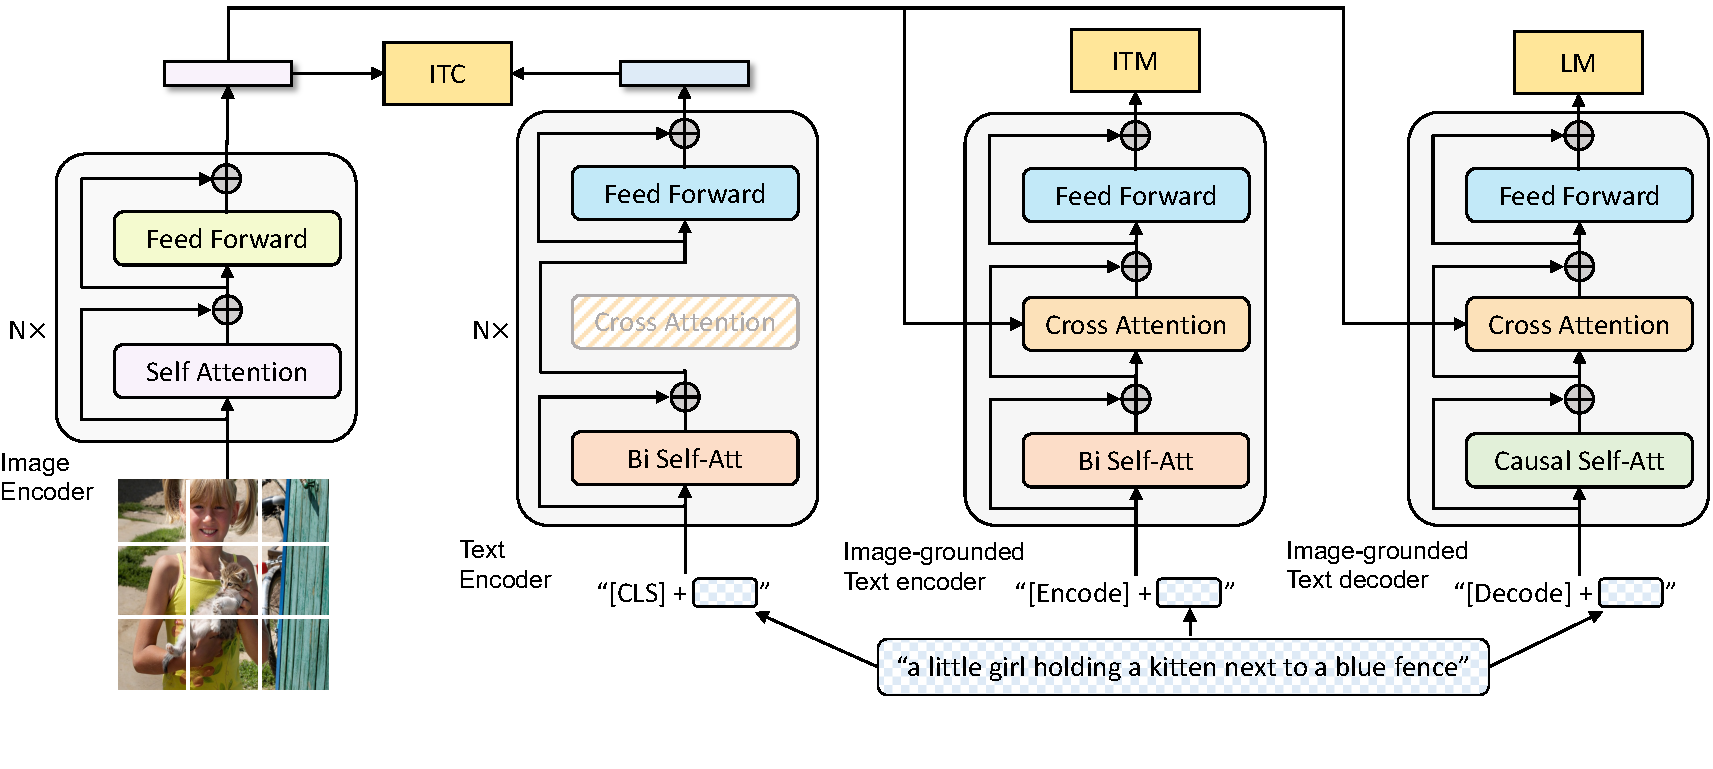
\includegraphics[width=0.98\textwidth]{imgs/MED.pdf}
\vspace{-6ex}
\caption{Pre-training model architecture and objectives of \name~(same parameters have the same color). We propose multimodal mixture of encoder-decoder, a unified vision-language model which can operate in one of the three functionalities:
(1) Unimodal encoder is trained with an image-text contrastive (ITC) loss to align the vision and language representations.
(2) Image-grounded text encoder uses additional cross-attention layers to model vision-language interactions,
and is trained with a image-text matching (ITM) loss to distinguish between positive and negative image-text pairs.
(3) Image-grounded text decoder replaces the bi-directional self-attention layers with causal self-attention layers,
and shares the same cross-attention layers and feed forward networks as the encoder. The decoder is trained with a language modeling (LM) loss to generate captions given images. 
}
\vspace{-2ex}
\label{fig:med}
\end{figure*}


\vspace{-0.5ex}
\subsection{Vision-language Pre-training}
\vspace{-0.5ex}
Vision-language pre-training (VLP) aims to improve performance of downstream vision and language tasks
by pre-training the model on large-scale image-text pairs.
Due to the prohibitive expense of acquiring human-annotated texts,
most methods~\cite{uniter,oscar,ALBEF,simvlm,clip} use image and alt-text pairs crawled from the web~\cite{CC,cc12m,align},
Despite the use of simple rule-based filters,
noise is still prevalent in the web texts.
However, the negative impact of the noise has been largely overlooked, shadowed by the performance gain 
obtained from scaling up the dataset.
Our paper shows that the noisy web texts are suboptimal for vision-language learning,
and proposes CapFilt that utilizes web datasets in a more effective way.

There have been many attempts to unify various vision and language tasks into a single framework~\cite{VLP,VL_T5,simvlm}.
The biggest challenge is to design model architectures that can perform both understanding-based tasks (\eg~image-text retrieval) and generation-based tasks (\eg~image captioning).
Neither encoder-based models~\cite{ALBEF,unimo,clip} nor encoder-decoder models~\cite{VL_T5,simvlm} can excel at both types of tasks,
whereas a single unified encoder-decoder~\cite{VLP} also limits the model's capability.
Our proposed multimodal mixture of encoder-decoder model offers more flexibility and better performance on a wide range of downstream tasks,
in the meantime keeping the pre-training simple and efficient.


\vspace{-1ex}
\subsection{Knowledge Distillation}
\vspace{-0.5ex}
Knowledge distillation (KD)~\cite{kd_hinton} aims to improve the performance of a student model by distilling knowledge from a teacher model.
Self-distillation is a special case of KD where the teacher and student have equal sizes.
It has been shown to be effective for image classification~\cite{noisy_student},
and recently for VLP~\cite{ALBEF}.
Different from mostly existing KD methods which simply enforce the student to have the same class predictions as the teacher,
our proposed CapFilt can be interpreted as a more effective way to perform KD in the context of VLP,
where the captioner distills its knowledge through semantically-rich synthetic captions,
and the filter distills its knowledge by removing noisy captions.

\vspace{-1ex}
\subsection{Data Augmentation}
\vspace{-0.5ex}
While data augmentation (DA) has been widely adopted in computer vision~\cite{DA_survey},
DA for language tasks is less straightforward.
Recently,
generative language models have been used to synthesize examples for various NLP tasks~\cite{DA,DA_AAAI,DA_QA,DA_commonsense}.
Different from these methods which focus on the low-resource language-only tasks,
our method demonstrates the advantage of synthetic captions in large-scale vision-language pre-training.

